%! Author = julianmour
%! Date = 01/05/2023

\section{Preliminary Results}
In this section, we describe our preliminary results.
We evaluate our approach on classifiers for the MNIST dataset, consisting of images showing a single digit.
The classifier's goal is to return the digit shown in the image. In our experiments, we focus on the global robustness property for the class $c=0,1,2$ and.

We consider two network architectures: 
a fully connected network consisting of three layers, ten neurons in each, denoted \texttt{3x10}, and a convolutional neural network. 
\ref{table_architectures} describes our models. For each model $F$, we define $F_1$ as $F$ and $F_2$ as $F$ with a slight change in a single weight in the last layer on $F$. Specifically we add a small addition to the weight between neuron $1$ in layer $L-1$ to neuron $3$ in layer $L$. We evaluate the algorithm across different weight additions. 
Furthermore we compare between 3 different approaches to show the scalability of our approach:
\begin{itemize}
    \item Baseline: the naive approach.
    \item VHAGaR extension.
    \item Our approach.
\end{itemize} 
We provide the MILP solver a timeout of 40800 seconds.

\begin{table}[H]
    \centering
    \resizebox{\textwidth}{!}{
    \begin{tabular}{@{\extracolsep{\fill}}llll@{}}
        \toprule
        \makecell{Dataset} & \makecell{Name} & \makecell{Architecture}  & \makecell{Iterations during training} \\
        \midrule            
        \multirow{2}{*}{MNIST} & 3 x 10 & 3 fully-connected layers & 20 \\
                               & CNN1 & 2 convolutional (stride 4) and 2 fully-connected layers & 20 \\
                               %& CNN2 & 2 convolutional (stride 4) and 2 fully-connected layers & 19 \\
        \bottomrule
    \end{tabular}
    }
    \caption{The networks used for this experience.
        \label{table_architectures}}
\end{table}

The examined perturbation is called brightness, where for a given $\epsilon$  %\Dana{what is the perturbation?}

Figure~\ref{fig:3_x_10}, Figure~\ref{fig:cnn0_1} and Figure~\ref{fig:cnn0_2} show the gaps in the execution time for the 3X10, CNN1, and CNN2 respectively.
Results show that our approach significant reduces the execution time, on average by 82\%. 
\begin{figure}[ht]
  \centering
  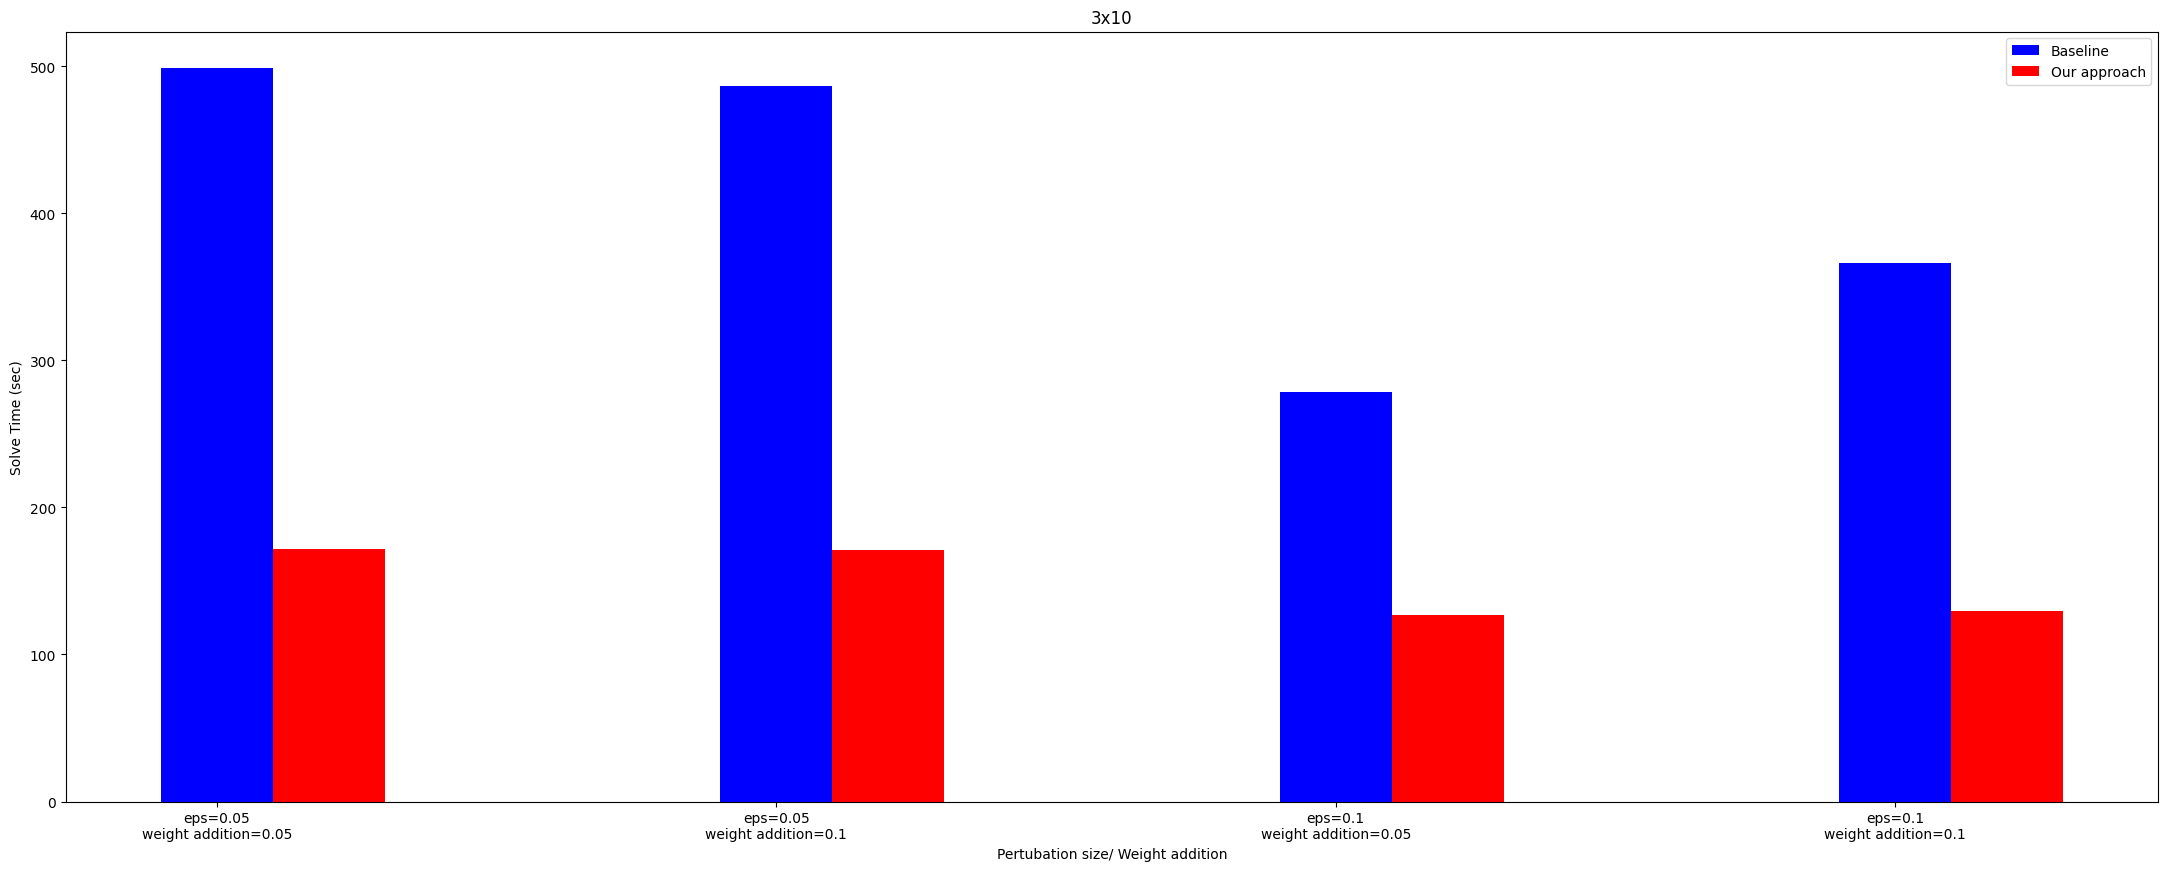
\includegraphics[width=0.95\textwidth]{3x10.png}
  \caption{The execution time of the baseline against our approach, when the model type is a fully connected network 3x10 .}
  \label{fig:3_x_10}
\end{figure}

\begin{figure}[ht]
  \centering
  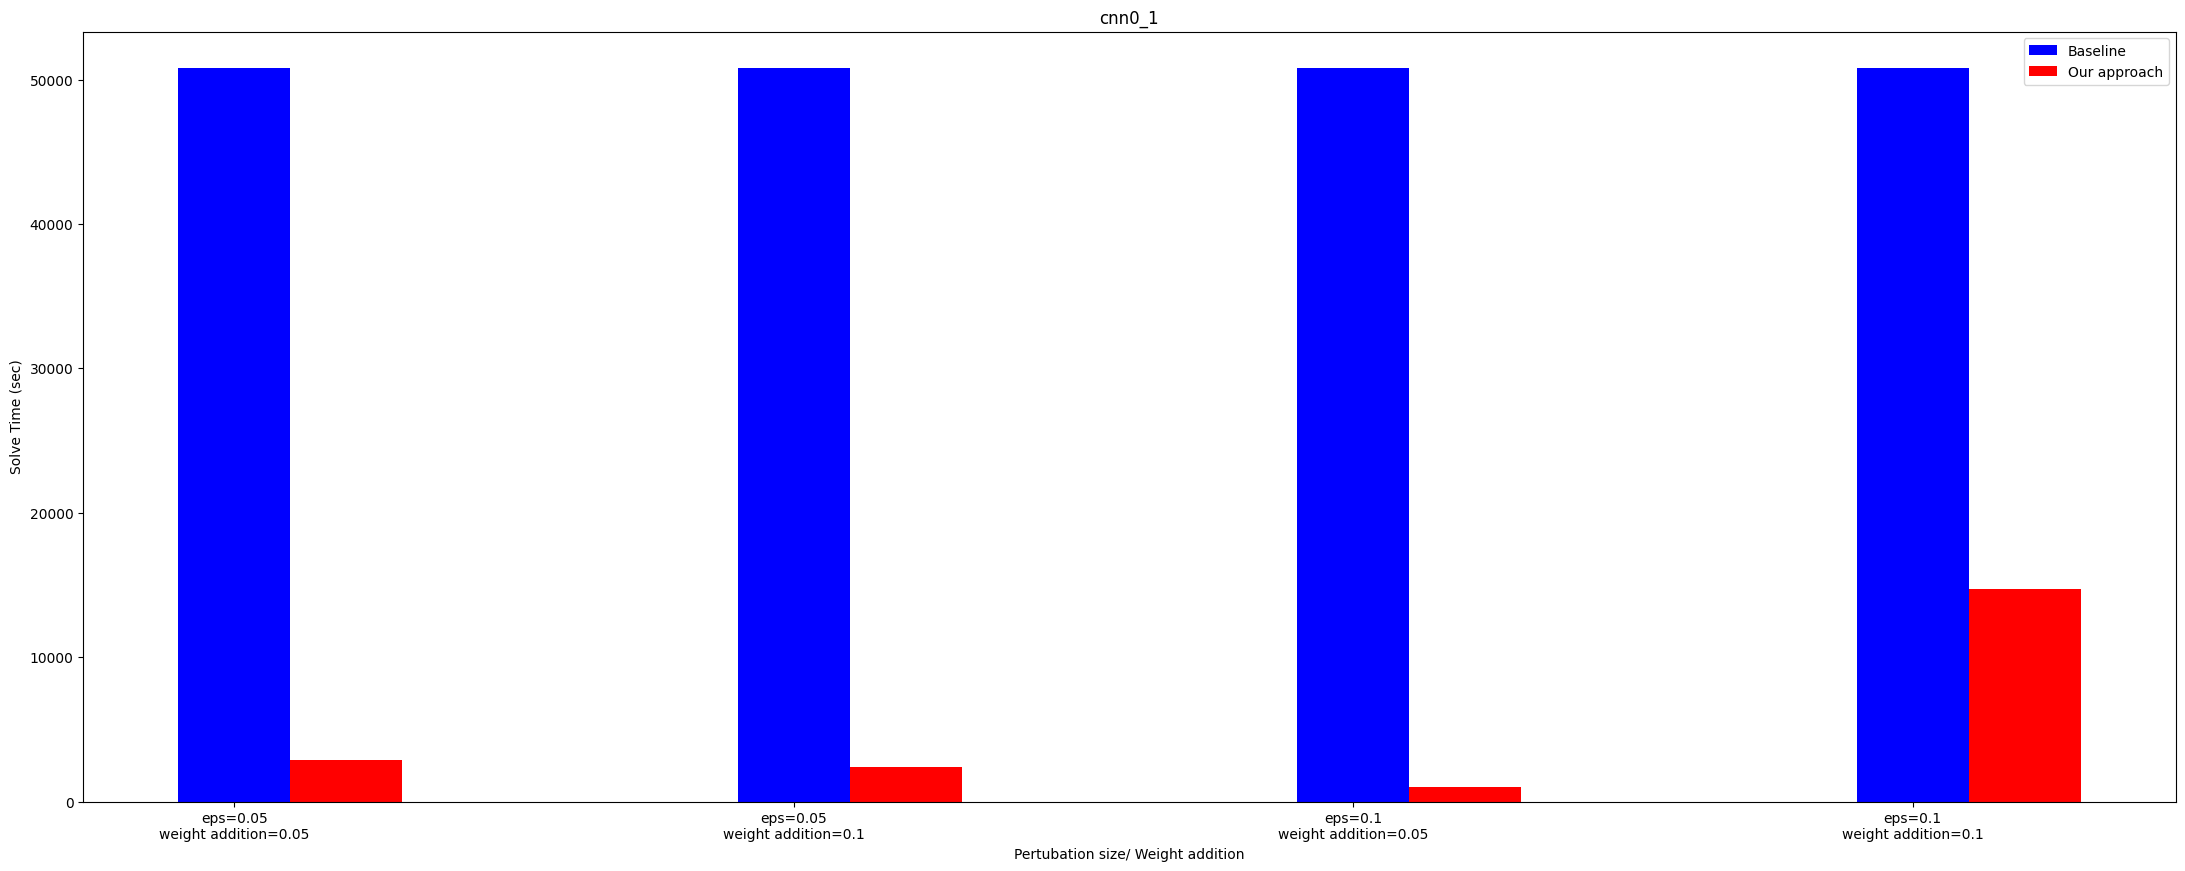
\includegraphics[width=0.95\textwidth]{cnn0_1.png}
  \caption{The execution time of the baseline against our approach, when the model type is a convolutional neural network, trained using 20 iterations\Dana{shortened it, call it for example conv-20}.}
  \label{fig:cnn0_1}
\end{figure}

\begin{figure}[ht]
  \centering
  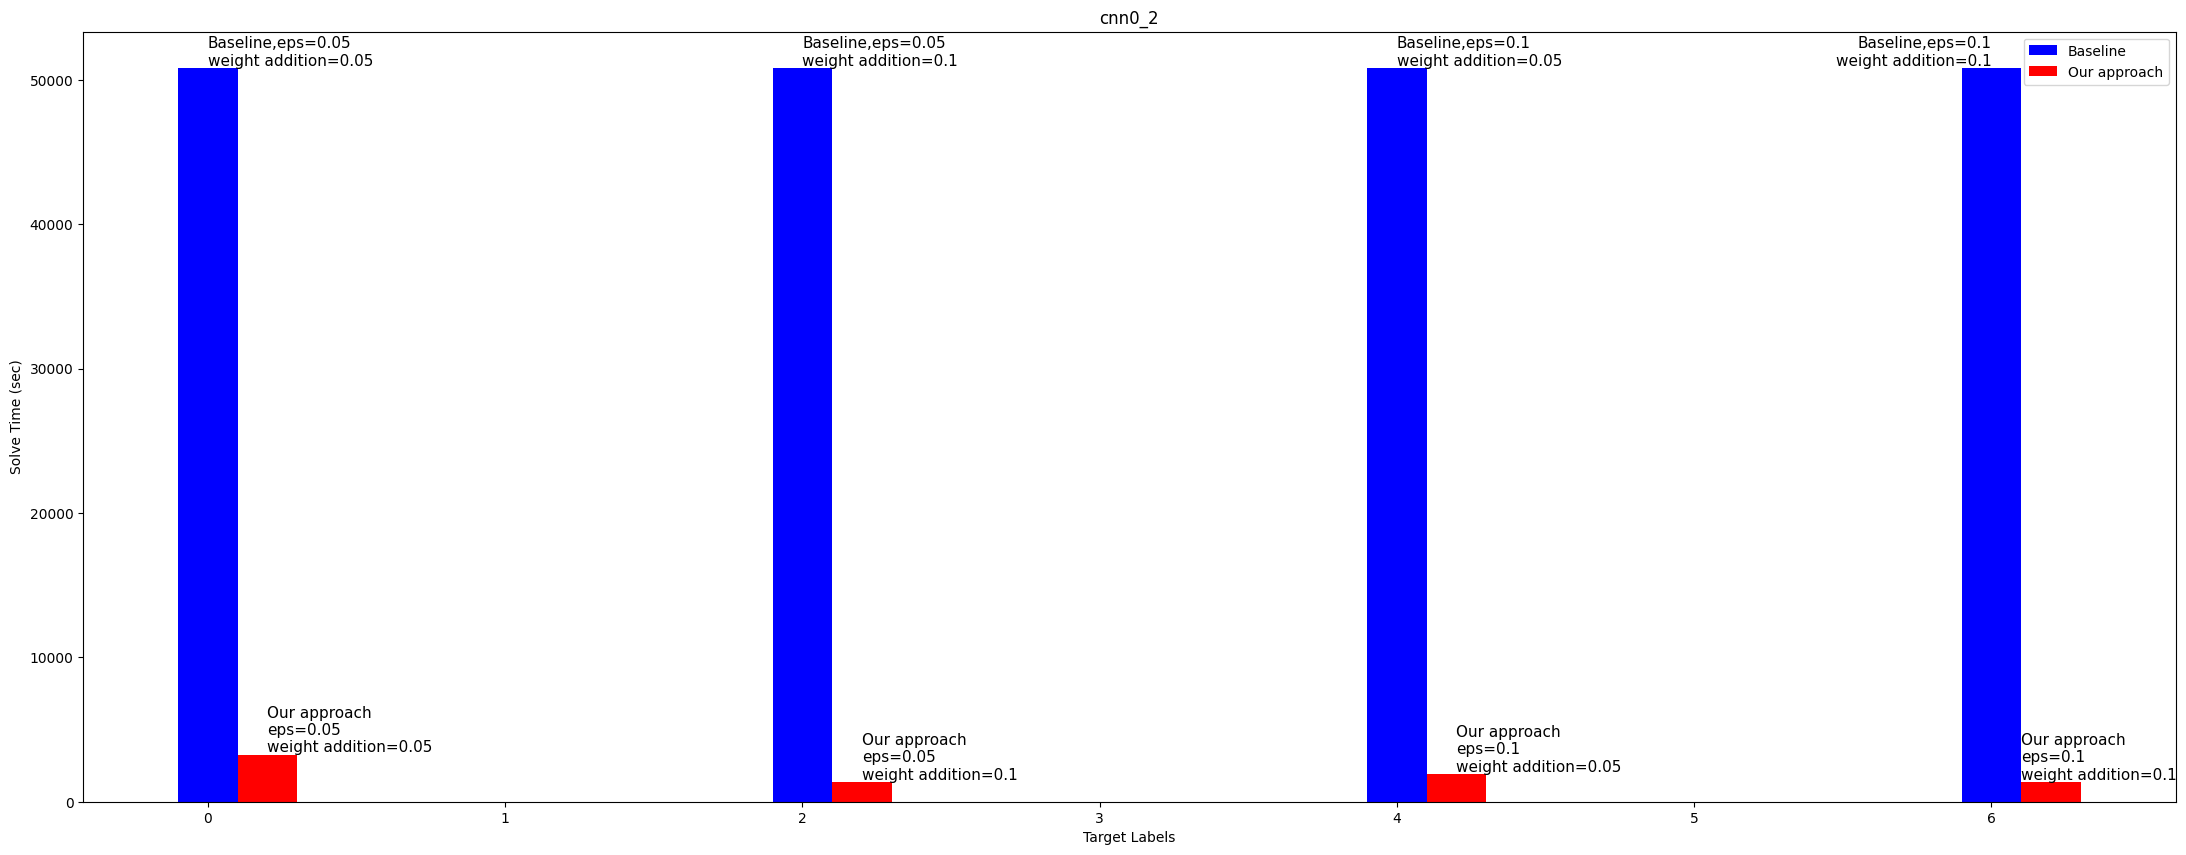
\includegraphics[width=0.95\textwidth]{cnn0_2.png}
  \caption{The execution time of the baseline against our approach, when the model type is a convolutional neural network, trained using 19 iterations .}
  \label{fig:cnn0_2}
\end{figure}

We next report the lower and upper bounds on $\delta_c$, computed within the timeout.
Table~\ref{table_3_x_10} shows the bounds for the \texttt{3x10} network. It shows that both approach obtain comparable bounds, with the baseline obtaining slightly tighter bounds. Table~\ref{table_cnn0_1} and Table~\ref{table_cnn0_2} show the results for the convolutional networks. Results show that our approach enables to improve tighter bounds by\Dana{complete}\%. %This is due to timeout. the base approach is much slower, and does not manage to find tighter bound for more complex architectures before reaching timeout. 
Namely, preliminary results show that our approach enhances scalability and consequently its accuracy. %is similar to the base approach for the tested scenario of two almost identical networks, besides a singular weight. Our goal is to further extend this improvement to other scenarios as well. 

\begin{table}[H]
	\centering
    \resizebox{\textwidth}{!}{
	\begin{tabular}{@{\extracolsep{\fill}}llllll@{}}
		\toprule
		& \makecell{ } & \makecell{Brightness[0.1] \\ Weight addition[0.1]} & \makecell{Brightness[0.1] \\ Weight addition[0.05]} & \makecell{Brightness [0.05] \\ Weight addition[0.1]} & \makecell{Brightness [0.05] \\ Weight addition[0.05]}\\
		\midrule			
		\multirow{2}{*}{Base approach} & upper bound  & 3.27 & 3.3 &  1.79 & 1.79\\
                              & lower bound & 3.27 & 3.27 &  1.79 & 1.79\\
		\midrule
		\multirow{2}{*}{Our approach} & upper bound  & 3.3 & 3.3 & 1.8 & 1.79\\
                              & lower bound & 3.27 & 3.27 & 1.79 & 1.79\\						
		\bottomrule
	\end{tabular}
}
\caption{The lower and upper bounds for 3X10 architecture 
		\label{table_3_x_10}}
\end{table}


\begin{table}[H]
	\centering
    \resizebox{\textwidth}{!}{
	\begin{tabular}{@{\extracolsep{\fill}}llllll@{}}
		\toprule
		& \makecell{ } & \makecell{Brightness[0.1] \\ Weight addition[0.1]} & \makecell{Brightness[0.1] \\ Weight addition[0.05]} & \makecell{Brightness [0.05] \\ Weight addition[0.1]} & \makecell{Brightness [0.05] \\ Weight addition[0.05]}\\
		\midrule			
		\multirow{2}{*}{Base approach} & upper bound  & 19.39 & 17.79 & 15.45 & 19.27\\
                              & lower bound & 15.01 & 15.01 &  12.18 & 12.19\\
		\midrule
		\multirow{2}{*}{Our approach} & upper bound  & 15.16 & 15.15 & 12.59 & 12.59\\
                              & lower bound & 15.01 & 15.01 &  12.46 & 12.46\\					
		\bottomrule
	\end{tabular}
}
\caption{The lower and upper bounds for CNN architecture with 20 iteration during training process.
		\label{table_cnn0_1}}
\end{table}


\begin{table}[H]
	\centering
    \resizebox{\textwidth}{!}{
	\begin{tabular}{@{\extracolsep{\fill}}llllll@{}}
		\toprule
		& \makecell{ } & \makecell{Brightness[0.1] \\ Weight addition[0.1]} & \makecell{Brightness[0.1] \\ Weight addition[0.05]} & \makecell{Brightness [0.05] \\ Weight addition[0.1]} & \makecell{Brightness [0.05] \\ Weight addition[0.05]}\\
		\midrule			
		\multirow{2}{*}{Base approach} & upper bound  & 15.77 & 17.71 & 15.6 & 19.16\\
                              & lower bound & 14.18 & 14.18 & 11.81 & 11.73\\
		\midrule
		\multirow{2}{*}{Our approach} & upper bound & 14.29 & 14.31 & 11.92 & 11.92\\
                              & lower bound & 14.15 & 14.17 & 11.8 & 11.81\\				
		\bottomrule
	\end{tabular}
}
\caption{The lower and upper bounds for CNN architecture with 19 iteration during training process.
		\label{table_cnn0_2}}
\end{table}
% NETA - image of database + explain: "hey we did good - but not good enough". 

% bounds in table
% times show in graph 